\documentclass[11pt,a4paper]{article}
\usepackage[a4paper,margin=2.4cm]{geometry}
\usepackage{fontspec}
\usepackage{amsmath,amssymb,amsthm}
\usepackage{unicode-math}
\setmainfont{Liberation Serif}
\setmonofont{DejaVu Sans Mono}[Scale=0.82]
\setmathfont{Latin Modern Math}
\usepackage{booktabs,longtable,array}
\usepackage{enumitem}
\setlist{nosep,leftmargin=2em}
\usepackage[hidelinks]{hyperref}
\usepackage{microtype}
\usepackage{graphicx}

\theoremstyle{plain}
\newtheorem{theorem}{Theorem}[section]
\newtheorem{lemma}[theorem]{Lemma}
\newtheorem{proposition}[theorem]{Proposition}
\theoremstyle{definition}
\newtheorem{definition}[theorem]{Definition}
\newtheorem{conjecture}{Conjecture}
\newtheorem{problem}{Problem}
\theoremstyle{remark}
\newtheorem*{example}{Example}

\newcommand{\Z}{\mathbb{Z}}
\newcommand{\lc}{\ell_{\mathrm{cell}}}
\newcommand{\lseg}{\ell_{\mathrm{seg}}}
\newcommand{\lean}[1]{\texttt{#1}}
\DeclareMathOperator{\vol}{vol}

\title{\textbf{The Relative Grid}\\[4pt] \large Main text, version 2.1}
\author{Muhammad Zafarov\thanks{Author of the system, its definitions and conjectures. Proofs and text prepared with the help of the AI assistant Claude (Anthropic). Text licensed under CC~BY~4.0, programs and Lean files under MIT. Repository: \url{https://github.com/abema2416-ops/Relative-Grid}.}}
\date{28 November 2026}

\begin{document}
\sloppy
\maketitle

\begin{abstract}
This is the canonical text of the ``Relative Grid'' system. It contains only the core of the system, the proven statements and explicitly marked conjectures. The working journal (draft 1.18, version history, all checks, in Russian) and a short paper (8 pages) are in the repository separately. The core consists of actions on finite sets of cells of the lattice $\Z^n$: stretching and compressing part of an object along one axis by an integer factor, deleting cells, gluing and ungluing side neighbours. Two measures are studied: the information loss of an action (in bits) and the number of actions needed to build a shape. Extensions (rotations, thin objects, gluings along edges and vertices, overlap outcomes) are moved to an appendix and marked as sketches.
\end{abstract}

\tableofcontents

\section{Introduction and status of results}

\paragraph{The question.} A shape cut by a grid is a set of cells. We fix a small set of actions on such sets and ask: how many actions are needed to build a given shape from one cell, and how much information is lost on the way.

\paragraph{What is specific to the system.} The action $\alpha$ itself is a special affine stretch (Theorem~\ref{thm:affine}); counting holes relies on cellular homology; stretching and compression resemble dilation and erosion in mathematical morphology. Specific to the system are: (1) how an action is specified — a zone and a fixed side, in cells; (2) bit-level loss for actions on shapes and the asymmetry ``removing is costly, restoring is free''; (3) gluings separated from touching, and their link to the number of holes; (4) the number of actions $\ell$, its NP-hardness for reliefs, its computability without loss, the rank bound and the segment rule. Related work is compared in §\ref{sec:related}.

\paragraph{How results are marked.} Table~\ref{tab:status} shows how each result is supported: \textbf{L} — machine-checked in Lean~4 (standard axioms only, no gaps); \textbf{L+T} — main part in Lean, the rest by a rigorous text proof; \textbf{T} — rigorous text proof; \textbf{K} — relies on a published theorem; \textbf{E} — exhaustive computer check only (not a proof).

\begin{longtable}{p{0.47\textwidth}cp{0.36\textwidth}}
\caption{Status of results}\label{tab:status}\\
\toprule
Result & Status & Where\\
\midrule
\endfirsthead
\toprule Result & Status & Where\\ \midrule \endhead
Properties of $\alpha$: cell count, no overlaps, merging within a block & L & §\ref{sec:props}\\
Stretching is lossless; preimages of $\sigma$ & L & §\ref{sec:props}\\
Shifting an object together with its zone & L & §\ref{sec:shift}\\
Every vanished cell costs $\ge1$ bit & L+T & §\ref{sec:loss}\\
Loss $\ge|A|-|B|$; removing costs $h$ bits, restoring 0 & L+T & §\ref{sec:loss}\\
Exact loss of compressing a row & T + E & §\ref{sec:loss}\\
Stretch = affine stretch & L & §\ref{sec:affine}\\
Limits of finite chains (stretches, compressions, $\sigma$) & T & §\ref{sec:affine}\\
Gluings and holes in the plane & L+T & §\ref{sec:holes}\\
$m(O)\le\lc(O)\le|O|-1$; a box in $k$ actions & L+T & §\ref{sec:count}\\
$\lc\le\ell\le\lc+2$; bounding box $+\sigma$ in $n+1$ & T & §\ref{sec:count}\\
Computability of $\ell$ without loss & L+T & §\ref{sec:count}\\
Reliefs: $R(H)$ and normal set basis, NP-hardness & L+T+K & §\ref{sec:reliefs}\\
Bounds and exact cases for $R(H)$ & L & §\ref{sec:reliefs}\\
Rank bound $R\ge\operatorname{rank}A$ & T & §\ref{sec:reliefs}\\
Where savings hide (tree method) & T & §\ref{sec:reliefs}\\
Computational method: 30/30 hard instances, instances with 150--257 heights & E & §\ref{sec:compute}\\
Segment rule: $\lseg\ge\ell_\alpha$; equality when $\ell_\alpha\le2$ & T & §\ref{sec:seg}\\
Segment rule in general & E & §\ref{sec:seg}, Conjecture~\ref{conj:seg}\\
Lower bound for reliefs & T (model) / E & §\ref{sec:reliefs}, Conjecture~\ref{conj:relief}\\
\bottomrule
\end{longtable}

\section{The core of the system}\label{sec:core}

\subsection{Cells, objects, shapes}

Notation: $e_1,\dots,e_n$ are the unit axis vectors; $|X|$ is the number of elements; $\|v\|_1=\sum|v_i|$; $c[i\mapsto v]$ is the cell $c$ with its $i$-th coordinate replaced.

\begin{definition}
A \emph{cell} is a point $c\in\Z^n$; it represents the cube $Q(c)=c+[0,1]^n$. Cells $c,c'$ are \emph{side neighbours} if $\|c-c'\|_1=1$. An \emph{object} is a pair $(O,S)$: $O\subset\Z^n$ finite and nonempty, $S$ a set of \emph{gluings}, i.e.\ unordered pairs of side neighbours in $O$. Neighbours without a gluing form a \emph{crack}. A \emph{piece} is a connected component of the gluing graph. A \emph{shape} is the class $[O]=\{O+v: v\in\Z^n\}$.
\end{definition}

\subsection{Actions}\label{sec:actions}

\begin{definition}[stretch and compression]\label{def:alpha}
Parameters: a finite zone $Z\subset\Z^n$, an axis $i$, a direction $s\in\{\pm1\}$, a factor $f\ge2$. Let $G=O\cap Z\ne\varnothing$, $a=\min\{sc_i:c\in G\}$ (the fixed side), $t(c)=sc_i-a$. Then
\begin{align*}
\alpha^{\uparrow}(O)&=(O\setminus G)\cup\{c[i\mapsto s(a+f\,t(c)+j)]: c\in G,\ 0\le j<f\},\\
\alpha^{\downarrow}(O)&=(O\setminus G)\cup\{c[i\mapsto s(a+\lfloor t(c)/f\rfloor)]: c\in G\}.
\end{align*}
\textbf{P3.} The action is admissible only if the new cells do not meet $O\setminus G$; otherwise it is rejected (the core has no parameter allowing overlaps).
\textbf{Gluings.} Under a stretch the $f$ image cells of one cell are glued consecutively, and a gluing $\{c,c'\}$ becomes gluings of all side-adjacent pairs of their images. Under a compression a gluing becomes the gluing of the images; if the cells merge, it disappears.
\textbf{P5.} An action after which glued cells would stop being side neighbours is inadmissible.
\end{definition}

\begin{definition}[$\sigma$, $\beta_\pm$]
$\sigma_Z(O)=O\setminus Z$ (gluings of deleted cells disappear). $\beta_+(K)$ adds to $S$ a nonempty set $K$ of unglued neighbouring pairs; $\beta_-(K')$ removes a nonempty $K'\subset S$. One application of $\beta$ is one action, however many pairs $K$ contains.
\end{definition}

\subsection{Loss and number of actions}

\begin{definition}[loss]
An action $\varphi$ with fixed $(Z,i,s,f)$ applies to any content of its zone. Loss is counted on cells:
\[
\lambda(\varphi,O)=\log_2\bigl|\{O'\subset\Z^n:\ O'\setminus Z=O\setminus Z,\ \varphi\text{ admissible on }O',\ \varphi(O')=\varphi(O)\}\bigr|.
\]
The loss of a chain is the sum of the losses of its steps. $\lambda(\beta_\pm)=0$: cells do not change, and on the pair $(O,S)$ with $K$ known the preimage is unique — $(O,S\setminus K)$ for $\beta_+(K)$ and $(O,S\cup K)$ for $\beta_-(K)$.
\end{definition}

\begin{definition}[number of actions]
A chain starts from one cell without gluings. For a set of actions $\mathcal A\subset\{\alpha^\uparrow,\alpha^\downarrow,\sigma,\beta_+,\beta_-\}$:
$\lc^{\mathcal A}(O)$ is the least length of a chain in $\mathcal A$ after which the set of cells equals $O$ (any gluings);
$\ell^{\mathcal A}(O,S)$ is the same with gluings exactly $S$.
Without an index the whole core is meant; $\ell_\alpha=\lc^{\{\alpha^\uparrow\}}$. The \emph{gluing cost} is the number of pairs glued by $\beta_+$ actions; it is not part of $\ell$.
\end{definition}

\subsection{Translation and zones}\label{sec:shift}

Zones are given in the coordinates of a specific representative of a shape. Shifting the object by $v$ shifts the zone with it.

\begin{proposition}[\lean{stretch\_shift}, \lean{shrink\_shift}, \lean{sigma\_shift}, \lean{anchor\_shift}]
$\alpha_{Z+v}(O+v)=\alpha_Z(O)+v$ (for stretches and compressions; the fixed side becomes $a+sv_i$) and $\sigma_{Z+v}(O+v)=\sigma_Z(O)+v$. Hence a chain can be shifted as a whole together with its zones; $\ell$ and $\lambda$ do not depend on the representative or the starting cell.
\end{proposition}

A zone not shifted with the object defines a different action: in general $\alpha_Z(O+v)\neq\alpha_Z(O)+v$.

\section{Basic properties of actions}\label{sec:props}

\begin{proposition}\label{prop:basic}
\begin{enumerate}[label=\upshape(\alph*)]
\item Cells outside the zone do not change; images keep all coordinates except the $i$-th (\lean{stretch\_keeps\_rest}, \lean{img\_r}).
\item Under an admissible stretch the images of distinct cells are disjoint and $|\alpha^\uparrow(O)|=|O|+(f-1)|G|$ (\lean{stretch\_card}, \lean{img\_inj}).
\item Under a compression two cells merge if and only if they lie in the same row and have the same $\lfloor t/f\rfloor$ (\lean{shrink\_merge}, \lean{shrinkCell\_eq\_iff}).
\item Stretching is lossless: two zone contents with the same result coincide (\lean{stretch\_lossless}).
\item $\sigma_Z(O')=\sigma_Z(O)$ if and only if $O'$ and $O$ agree outside $Z$; hence $\lambda(\sigma_Z)=|Z|$ (\lean{sigma\_preimage}).
\end{enumerate}
\end{proposition}

\begin{proposition}[what each core action preserves]
\begin{center}
\begin{tabular}{lccc}
\toprule
& cells & pieces & holes $d$ ($n=2$)\\
\midrule
$\alpha^\uparrow$ & $+$ & unchanged & unchanged\\
$\alpha^\downarrow$ & $-$ & may change & may change\\
$\beta_+$ & unchanged & $-1$ or $0$ & $+1,0,-1$\\
$\beta_-$ & unchanged & $+1$ or $0$ & $+1,0,-1$\\
$\sigma$ & $-$ & may change & may change\\
\bottomrule
\end{tabular}
\end{center}
\end{proposition}
\begin{proof}
Stretch: gluings map to gluings, no new gluings between pieces appear, P5 forbids breaking; holes — Theorem~\ref{thm:holes}(b). A gluing joins two cells of one or two pieces. Compression and $\sigma$ — examples: two unglued neighbouring cells compressed twofold give one; a $3\times3$ ring compressed threefold along a row loses its hole.
\end{proof}

\section{Information loss}\label{sec:loss}

\begin{lemma}\label{lem:bit}
If an action decreases the number of cells by $d>0$, its loss is at least $d$ bits.
\end{lemma}
\begin{proof}
For $\sigma$ — Proposition~\ref{prop:basic}(e). Let the action be a compression; nonempty blocks $B_0$ (containing the cell $e$ attaining $a$), $B_1,\dots,B_r$, with $m_B$ group cells in block $B$, $d=\sum(m_B-1)$. Consider objects $O'$ agreeing with $O$ outside $Z$ with $O'\cap Z\subset G$, $e\in O'$ and every $B_k$ nonempty. (1) The fixed side is the same (\lean{anchor\_of\_subset}). (2) The result is the same (\lean{shrink\_same\_of\_blocks}). (3) The new cells are a subset of the old ones, so P3 holds. (4) Choices in different blocks are independent: in $B_0$ the cell $e$ is forced ($2^{m_{B_0}-1}$ variants), in $B_k$ any nonempty subset ($2^{m_{B_k}}-1$). (5) $2^{m_0-1}\prod(2^{m_k}-1)\ge2^d$ (\lean{loss\_ge\_bits\_anchor}).
\end{proof}

\begin{theorem}\label{thm:loss}
(a) In any transformation $A\to B$ the loss is at least $|A|-|B|$ bits. (b) If $A$ is side-connected, $B=A\setminus H\ne\varnothing$, $|H|=h$, then the least loss of $A\to B$ is $h$ bits and that of $B\to A$ is zero. (c) For side-connected $B$ the least loss of $A\to B$ lies between $\max(0,|A|-|B|)$ and $|A|-1$.
\end{theorem}
\begin{proof}
(a) Sum Lemma~\ref{lem:bit} over the steps. (b) $h$ is attained by $\sigma_H$. Conversely, every component of $H$ borders $B$ along a side, so the cells of $H$ can be ordered so that each neighbours an already built one; each is restored by stretching a neighbour twofold towards it (\lean{grow\_one}), without loss (\lean{stretch\_lossless}). (c) Upper bound: $\sigma$ leaves one cell ($|A|-1$ bits), then lossless growth (Theorem~\ref{thm:bounds}).
\end{proof}

\begin{theorem}[exact loss of compressing a row]\label{thm:exact}
Let the zone be a row segment with positions $0,\dots,L-1$, $a$ the least occupied position, compressed by $f$; positions $a,\dots,L-1$ split into blocks by $\lfloor(p-a)/f\rfloor$, $z_B$ is the number of zone positions in block $B$, $B_0$ the anchor's block. Then the number of zone contents with the same result is
\[
N=2^{\,z_{B_0}-1}\prod_{B\ne B_0,\ B\text{ nonempty}}\bigl(2^{z_B}-1\bigr).
\]
\end{theorem}
\begin{proof}
The result is determined by the anchor and the set of nonempty blocks. A content gives the same result exactly when its leftmost cell is $a$ and the same blocks are nonempty. Choices in blocks are independent.
\end{proof}
Checked exhaustively on 2872 random rows ($L\le13$, $f=2,3,4$). Example: $L=20$, $f=2$, four cells vanish — the lemma gives $N\ge16$, the theorem $N=4374$.

\begin{example}
A row of 4 cells $\{0,1,2,3\}$ compressed twofold: blocks $\{0,1\}$ and $\{2,3\}$, result $\{0,1\}$. Preimages: cell $0$ forced, cell $1$ free ($2$ variants), from $\{2,3\}$ any nonempty subset ($3$ variants); $N=6$, loss $\log_2 6\approx2.58$ bits for two vanished cells.
\end{example}

\begin{figure}[h]\centering
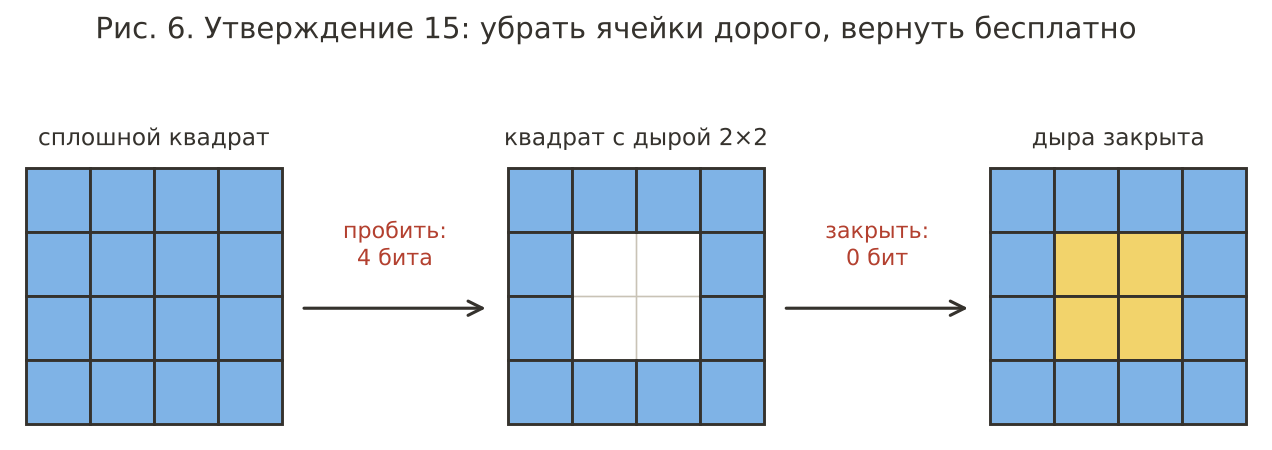
\includegraphics[width=0.8\textwidth]{fig6.png}
\caption{Theorem~\ref{thm:loss}(b): punching a hole of 4 cells costs 4 bits, closing it costs 0 bits. (Labels in Russian.)}
\end{figure}

\section{Relation to continuous geometry}\label{sec:affine}

Let $F(O)=\bigcup_{c\in O}Q(c)$, $y=sx_i$, $T\colon y\mapsto a+f(y-a)$.

\begin{theorem}\label{thm:affine}
(a) $F(\alpha^\uparrow(O))=F(O\setminus G)\cup T(F(G))$ exactly (\lean{T\_cell}, \lean{block\_eq\_cells}). (b) $\alpha^\downarrow(O)=(O\setminus G)\cup\{c:\vol(Q(c)\cap T^{-1}F(G))>0\}$ (\lean{shrink\_slab}).
\end{theorem}
\begin{proof}
(a) The cell at position $p=a+t$ goes to cells $a+ft,\dots,a+ft+f-1$, which occupy $T([p,p+1))$. (b) $T^{-1}$ maps a cell to a slab of thickness $1/f$ inside the cell $a+\lfloor t/f\rfloor$.
\end{proof}

\begin{figure}[h]\centering
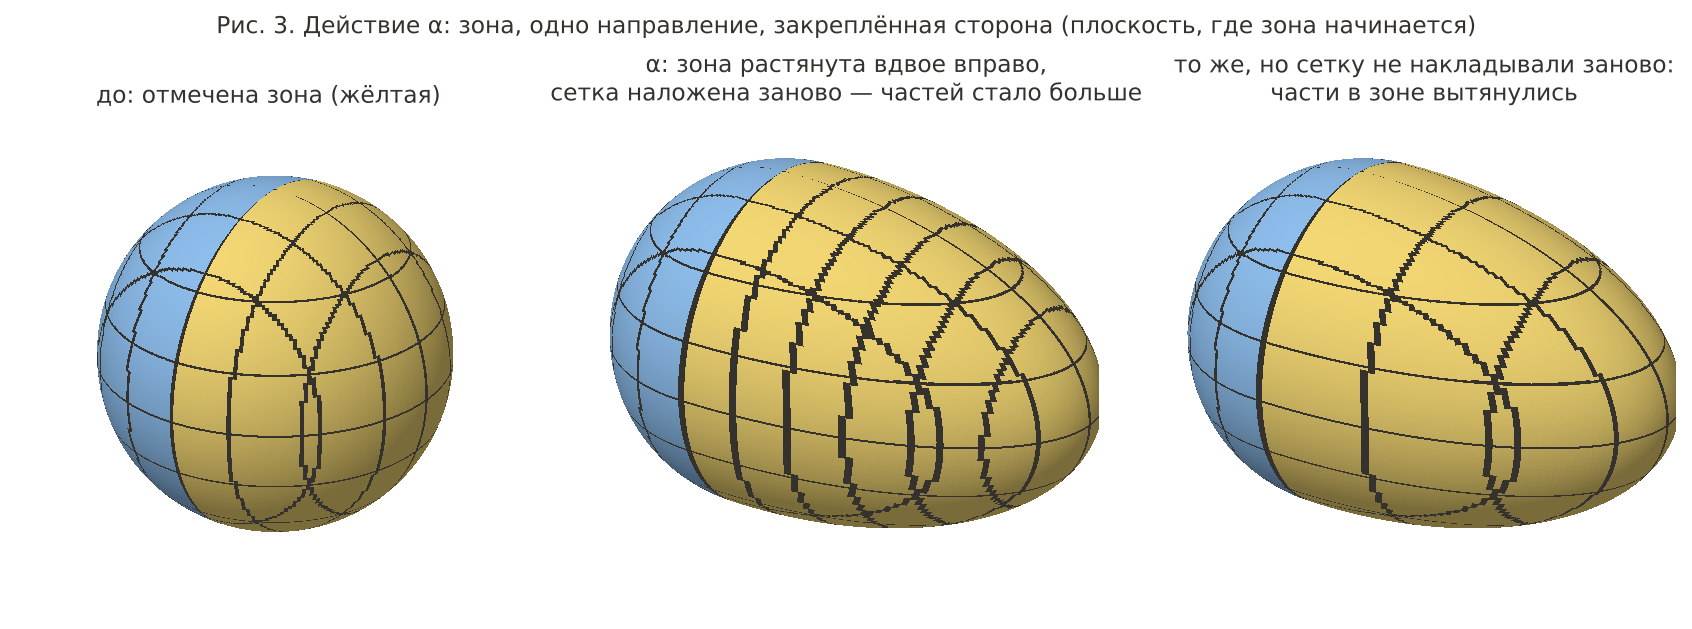
\includegraphics[width=0.9\textwidth]{fig3.png}
\caption{The action $\alpha$ on a ball: the zone is stretched twofold from its fixed side. Left to right: zone marked; stretched and re-cut by the grid; the same without re-cutting. By Theorem~\ref{thm:affine} both pictures show the same shape $T(F(G))$.}
\end{figure}

\paragraph{Limits.} The record of a shape $F$ at level $N$ is the set of level-$N$ cells in which $F$ occupies a fraction at least $\theta\in(0,1]$ (or a positive fraction for $\theta=0^+$).

\begin{theorem}[records of one shape]\label{thm:rec}
If $F$ is bounded and Jordan measurable, its records converge to $F$ in volume, and their roundings at each fixed level stabilize for $\theta=0^+$ always and for $\theta\in(0,1]$ for all thresholds except at most countably many.
\end{theorem}
\begin{proof}
Wrong cells meet $\partial F$, and their total volume tends to zero. The fraction of the record in each coarse cell converges to that of $F$; rounding stabilizes unless this fraction equals $\theta$. There are countably many pairs (level, cell).
\end{proof}

\begin{theorem}[finite chains]\label{thm:limit}
Let on levels $N_1\mid N_2\mid\cdots$ the records $O_N$ and groups $G_N$ converge in volume to bounded $F\supset K$, with $K$ Jordan measurable, and anchors $a_N/N\to A$. Then the stretches $\alpha^\uparrow(O_N)$ converge to $(F\setminus K)\cup T_A(K)$, the compressions $\alpha^\downarrow(O_N)$ to $(F\setminus K)\cup T_A^{-1}(K)$, and $\sigma_{Z_N}(O_N)$ with $F(O_N\cap Z_N)\to W$ to $F\setminus W$. The same holds for any finite chain if the group limits of all compressions are Jordan measurable.
\end{theorem}
\begin{proof}
Stretch: by Theorem~\ref{thm:affine}(a); $T$ multiplies volume by $f$, and a small anchor shift gives a small error. Compression: let $B(X)$ be the compression of a cell set $X$ with anchor $a_N$, $K_N$ the record of $K$. (1) $|B(G_N)\triangle B(K_N)|\le|G_N\triangle K_N|$: a block in the difference contains a cell of the difference, distinct blocks distinct cells. (2) $F(B(K_N))\supseteq T^{-1}F(K_N)$; excess volume comes only from incomplete blocks, each containing adjacent cells in and out of $K_N$ whose union meets $\partial K$, and there are $o(N^n)$ such cells. (3) $\vol(T^{-1}F(K_N)\triangle T^{-1}K)=\vol(F(K_N)\triangle K)/f\to0$. Unions and differences — by the symmetric-difference inequality.
\end{proof}

\section{Gluings and holes in the plane}\label{sec:holes}

Let $n=2$. The complex $K(O,S)$: one square per cell, common sides of glued pairs identified. The number of holes is $d=\dim H_1(K;\mathbb Q)$; $q$ is the number of lattice points surrounded by a fully glued $2\times2$ square.

\begin{theorem}\label{thm:holes}
(a) $d=(\text{number of pieces})-|O|+|S|-q$. (b) An admissible stretch does not change $d$. (c) One gluing changes $d$ by $+1$, $0$ or $-1$. (d) Building an object by stretches and gluings needs at least $d$ glued pairs; if $q=0$, exactly $d$ pairs suffice.
\end{theorem}
\begin{proof}
(a) Faces $|O|$, edges $4|O|-|S|$. Over a point $p$ the graph $\Gamma(p)$ (squares with corner $p$; glued sides ending at $p$) is a subgraph of a 4-cycle; the number of vertices of $K$ over $p$ is the number of its components $k-s+[\text{cycle}]$ (\lean{vertex\_count}). Hence $\chi=|O|-|S|+q$ (\lean{euler}). By rank–nullity $\chi=b_0-b_1+b_2$. $b_2=0$: in a nonzero 2-cycle take a square with nonzero coefficient and lexicographically largest cell; its right side is shared only with the square to its right, whose coefficient is $0$ — a contradiction. The components of $K$ are the pieces.
(b) Cells $+(f-1)|G|$, gluings $+(f-1)|G|+(f-1)r$ ($r$ — gluings inside $G$ across the axis), $q$ grows by $(f-1)r$, pieces unchanged (\lean{stretch\_keeps\_d}). (c) A gluing inside a piece: $|S|+1$, $q+\{0,1,2\}$; between pieces: one piece fewer, $q$ unchanged (\lean{glue\_inside}, \lean{glue\_join}, \lean{three\_seams\_connect}). (d) From (b), (c) (\lean{d\_le\_glues}); upper bound — growth along a spanning tree of the gluing graph plus $|S|-|O|+1$ gluings.
\end{proof}

Consequence: a hole can appear in two ways — by gluing (0 bits) or by punching (at least a bit per cell).

\begin{figure}[h]\centering
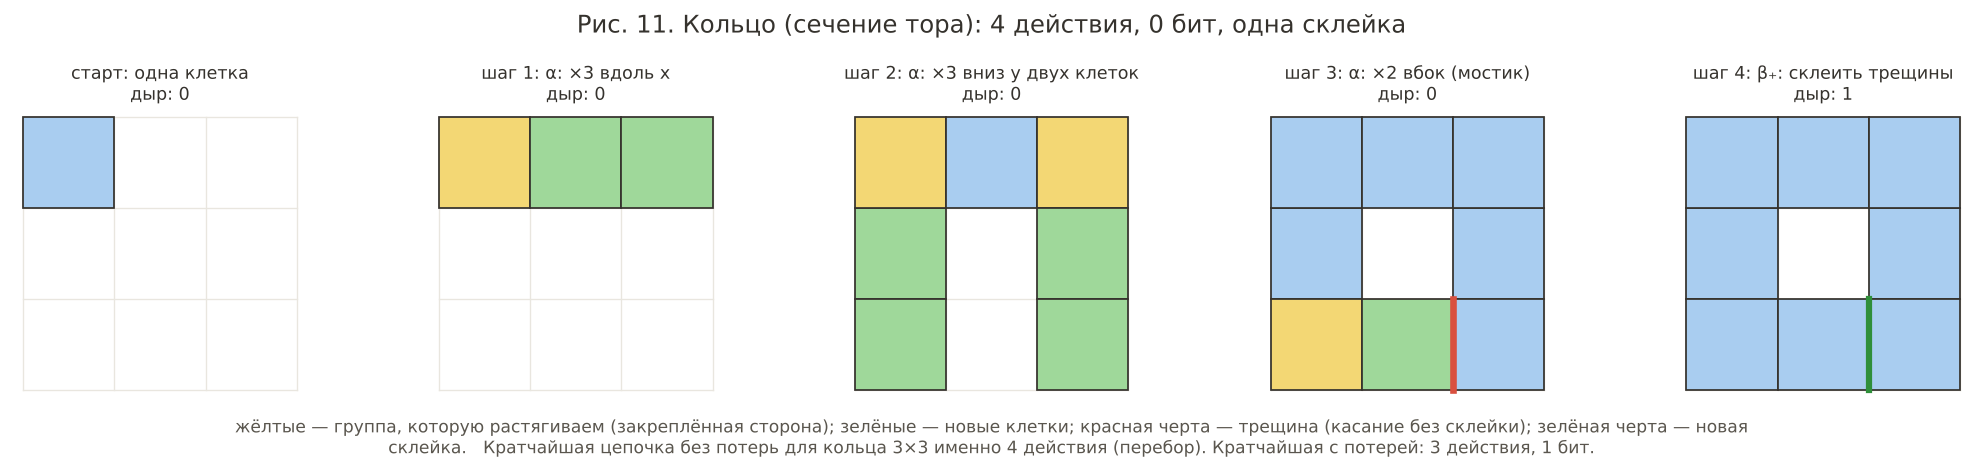
\includegraphics[width=\textwidth]{fig11a.png}
\caption{A $3\times3$ ring without loss: three stretches and one gluing. Stretches do not create the hole (Theorem~\ref{thm:holes}(b)); it is closed by gluing the crack. With loss the ring is built in 3 actions ($3\times3$ square and $\sigma$ of the centre, 1 bit). (Labels in Russian.)}
\end{figure}

\begin{example}
A $3\times3$ ring with all 8 joints glued: $d=1-8+8-0=1$. Without one joint: $d=0$ (a crack in the ring). A $2\times2$ square with all joints glued: $d=1-4+4-1=0$. A $2\times3$ rectangle without the middle inner joint: $d=1-6+6-0=1$ — the inner crack counts as a hole.
\end{example}

\begin{theorem}[a lossless hole requires gluing]
If a chain from one cell builds an object with $d\ge1$, it contains $\beta_+$, $\beta_-$, a $\sigma$ removing a cell, or a compression with merging.
\end{theorem}
\begin{proof}
Stretches do not change $d$; a compression without merging is an isomorphism of gluing graphs preserving fully glued squares, so it does not change $d$ either. One cell has $d=0$.
\end{proof}

\section{The number of actions}\label{sec:count}

Let $m(O)$ be the number of axes along which the cells of $O$ have two distinct coordinate values.

\begin{theorem}\label{thm:bounds}
(a) $m(O)\le\lc(O)$ for every object and every chain in the core (\lean{axes\_le\_length}). (b) If $O$ is side-connected, $\ell_\alpha(O)\le|O|-1$, with a lossless chain. (c) A box with sides $\ge2$ along $k$ axes: $\lc=k$, and also $k$ with all neighbour gluings. (d) $\lc(O)\le\ell(O,S)\le\lc(O)+2$. (e) If $\sigma$ is allowed, $\lc(O)\le n+1$ for every $O$, and such a chain loses $|P|-|O|$ bits ($P$ — the smallest box containing $O$).
\end{theorem}
\begin{proof}
(a) Values of the $i$-th coordinate grow only under $\alpha$ along axis $i$; formally — \lean{step\_spreads}, \lean{chain\_spreads}. (b) Breadth-first traversal of the neighbour graph; each step — \lean{grow\_one}. (c) One stretch per axis; stretches glue all side neighbours by themselves. (d) Append $\beta_-(S'\setminus S)$ and $\beta_+(S\setminus S')$. (e) A bounding box in $\le n$ stretches and $\sigma_{P\setminus O}$ with $2^{|P\setminus O|}$ preimages.
\end{proof}

\begin{example}
An $m\times m\times m$ cube from one cell: a stretch by $m$ along each axis, $\lc=3$ for every $m\ge2$ (no fewer by (a)). An L-shape of 5 cells in the plane: a row of 3 cells, then the end cell upward by 3 — 2 actions, $m=2$, bound (a) is tight. A $3\times3$ ring: $\ell_\alpha=3$, but a ring with glued joints needs one more $\beta_+$, $\ell=4$; with $\sigma$ — 3 actions and 1 bit.
\end{example}

Part (e) is a trade of work for loss: any shape in $n+1$ actions, but with a bit per cut-out cell.

\begin{theorem}[computability without loss]\label{thm:dec}
For $\mathcal A=\{\alpha^\uparrow\}$ and $\mathcal A=\{\alpha^\uparrow,\beta_\pm\}$ the numbers $\lc^{\mathcal A}(O)$ and $\ell^{\mathcal A}(O,S)$ are computable.
\end{theorem}
\begin{proof}
(1) The bounding box never shrinks under stretching, so all intermediate shapes lie in the final bounding box (\lean{stretch\_frame}, \lean{schain\_frame}). (2) The number of cells does not decrease (\lean{stretch\_card}). (3) The factor is at most a side of the box (\lean{stretch\_image\_ends}). (4) The result depends only on $G=O\cap Z$, the axis, the direction and $f$. Hence there are finitely many states and transitions, and breadth-first search terminates.
\end{proof}

Consequence: all searches in bounded boxes in §\ref{sec:seg} are exact. With compressions and $\sigma$ a shape may leave the box, and the question is open (Problem~\ref{pr:dec}).

\section{Reliefs and hardness of counting}\label{sec:reliefs}

A relief: a base $B\subset\Z^{n-1}$, heights $h\colon B\to\{1,2,\dots\}$, $O=\{(b,j):0\le j<h(b)\}$. In the \emph{column model} the base is built first, then zones of whole columns are stretched upward; a height is the product of factors. $H$ is the set of heights greater than 1, $D=|H|$, $R(H)$ the least number of factors such that every height is a product of a subset of them. Then $\ell(O)\le\ell(B)+R(H)$.

\begin{theorem}[candidates]\label{thm:cand}
There is a minimum set of factors in $C(H)=H\cup\mathcal D\cup\mathcal Q$, where $\mathcal D$ are the numbers $\ge2$ dividing two heights and $\mathcal Q=\{h/d\ge2: d\in\mathcal D,\ d\mid h\}$.
\end{theorem}
\begin{proof}
A factor shared by two heights lies in $\mathcal D$. A height has at most one private factor (two are replaced by their product, \lean{step2}). The private factor of $h$ is replaced by $h/a$ if a shared factor $a$ occurs in the factorization of $h$ (\lean{step3}), otherwise by $h$.
\end{proof}

\begin{theorem}\label{thm:R}
(a) $\lceil\log_2(D+1)\rceil\le R\le D$ (\lean{card\_le\_pow}). (b) Pairwise coprime heights: $R=D$ (\lean{coprime\_R\_eq\_D}). (c) $H=\{b,\dots,b^D\}$: $R=\lceil\log_2(D+1)\rceil$ (\lean{ladder\_exact}). (d) For fixed $k$ the condition $R\le k$ is checkable in time polynomial in $D$ and the largest height.
\end{theorem}
\begin{proof}
(a) $R$ factors give $\le2^R-1$ nonempty subsets. (b) A shared factor would divide both heights. (c) Binary expansion of the exponent. (d) Enumerate sets of $k$ candidates from Theorem~\ref{thm:cand}.
\end{proof}

\begin{theorem}[NP-hardness]\label{thm:np}
For squarefree heights $R(H)$ equals the least size of a normal set basis of the family of sets of prime divisors of the heights. Hence ``$R(H)\le K$?'' is NP-hard with heights written in binary.
\end{theorem}
\begin{proof}
Parts of a factorization of a squarefree height are squarefree and pairwise have no common divisor greater than 1 (\lean{sqfree\_dvd}, \lean{sqfree\_parts\_disjoint}), so their prime sets are disjoint. Conversely, a basis yields products of primes. A family of subsets of $\{u_1,\dots,u_k\}$ is encoded by the first $k$ primes; the heights have polynomial length. Normal Set Basis is NP-complete \cite{jiang}.
\end{proof}

\paragraph{The exponent table.} Let $A$ be the table whose row is a height, column a prime, and entry the exponent of the prime in the height. A factor is a ``rectangle'' in this table: the heights using it $\times$ its exponents.

\begin{theorem}[rank bound]\label{thm:rank}
$R(H)\ge\operatorname{rank}_{\mathbb Q}A$.
\end{theorem}
\begin{proof}
If the heights are built from factors $m_1,\dots,m_R$, the exponent vector of $h$ equals $\sum_{m\in S_h}v(m)$. Hence $A=UV$ with $U$ a $0/1$ table of size $|H|\times R$ and $V$ the exponent table of the factors. The rank of a product is at most $R$.
\end{proof}

The lower bound is $\max(\operatorname{rank}A,\lceil\log_2(D+1)\rceil)$: the logarithm is strong when there are many heights, the rank when there are many primes. If it meets any upper bound ($D$, the number of primes, or the answer of any heuristic), the answer is exact without search.

\begin{theorem}[where savings hide]\label{thm:tree}
Let a set $B$ build $H$; call a factor shared if it occurs in the factorizations of at least two heights, and private otherwise; let $T$ be the heights factored only by shared factors. Then $|B|\ge(\text{number of shared})+(|H|-|T|)$, and every factor in the factorization of $h\in T$ lies in $h\cap g$ for some other height $g$. If $R(H)<|H|$, there is a group $T$ with $R(T)<|T|$; its rows in $A$ are linearly dependent. If $A$ has exactly one row dependency, $T$ contains its support.
\end{theorem}
\begin{proof}
Each height outside $T$ uses at least one private factor, and private factors of different heights are different. A shared factor occurring in $h$ and in $g$ lies in $h\cap g$. From $R(T)<|T|$ and Theorem~\ref{thm:rank}, $\operatorname{rank}(T)<|T|$; a dependency among the rows of $T$ extends by zeros to one among the rows of $H$, i.e.\ is a multiple of the unique one.
\end{proof}

\begin{example}
An instance with 12 heights (12 primes, rank 11): the unique row dependency covers 9 heights, so only the 8 groups containing these 9 need checking. None can be built with a saving, hence $R=12$. Full search would need about $2\cdot10^{20}$ checks; this route needed about $6\cdot10^7$.
\end{example}

\begin{theorem}[lower bound in the column model]
If the base of a planar relief has at least two cells, then in the column model $\ell\ge1+\lceil\log_2D'\rceil$, where $D'$ is the number of distinct heights.
\end{theorem}
\begin{proof}
The base needs at least one action (Theorem~\ref{thm:bounds}(a)); there are at least $\lceil\log_2(D+1)\rceil$ factors (Theorem~\ref{thm:R}(a)), $D'\le D+1$.
\end{proof}

\begin{example}
Heights $\{2,3,6\}$: factors $2$ and $3$ give $2$, $3$ and $6=2\cdot3$, so $R=2=\lceil\log_2 4\rceil$ — the lower bound is tight. Heights $\{2,3,5\}$ are coprime: $R=3$. Heights $\{2,4,8,16\}$: factors $2,4$ give only $2,4,8$, so one more is needed; $R=3$.
\end{example}

\begin{conjecture}\label{conj:relief}
The same bound holds for arbitrary chains of stretches (with parts of columns, where heights add). Checked exhaustively on 1307 reliefs.
\end{conjecture}

\subsection{Computational method}\label{sec:compute}
For practical computation of $R(H)$ the following procedure is used: (1) factor the heights and merge primes with identical occurrence patterns; (2) recognize a pattern — pairwise coprime heights ($R=D$), a ladder of powers ($R=\lceil\log_2(D+1)\rceil$); (3) lower bound $L=\max(\operatorname{rank}A,\lceil\log_2(D+1)\rceil)$; (4) heuristics — counting, prime patterns, \emph{jumps} (the most frequent ratios $b/a$ of heights), \emph{common divisors} (greedily extract the common part $g$ with the largest saving $(u-1)(k-1)$, where $u$ is the number of heights from which it can be cut out and $k$ the number of primes in $g$); the best gives an upper bound $U$; (5) if $U>L$, exact search from $L$ with rank pruning; (6) Theorem~\ref{thm:tree}; (7) write each height as a product of the factors found and verify.

Results (programs in the repository): all 30 hard test instances solved exactly; an instance with 257 heights of up to 32 digits (9 hidden factors) in 0.02~s via jumps; an instance with 150 heights of up to 36 digits with no jumps or patterns (60 hidden factors) in 1.2~s via common divisors, the answer matching the rank and hence exact. There are also instances with only 20 heights and strongly overlapping hidden factors where a gap $12\le R\le14$ remains after a minute. This agrees with NP-hardness: each method is strong on its own family, and no universal fast method has been found.

\section{The segment rule}\label{sec:seg}

A \emph{segment} of an object along axis $i$ is a maximal run of consecutive cells. A \emph{segment step} (axis $i$ and direction $s$ fixed): \emph{multiply} — stretch by $f\ge2$ the union of several segments from different lines with a common start; \emph{extend} — stretch by $a+1$ the end cells of several segments from different lines with a common end. $\lseg(O)$ is the least number of such steps.

\begin{theorem}\label{thm:seg}
(a) $\lseg(O)\ge\ell_\alpha(O)$ for every $O$. (b) If $\ell_\alpha(O)\le2$, then $\lseg(O)=\ell_\alpha(O)$ in every dimension.
\end{theorem}
\begin{proof}
(a) Every step is a special case of $\alpha^\uparrow$. (b) After one step the object is a row $R$ along axis $i$. A second step along an axis $j\ne i$: the anchor is common, $t=0$ for all group cells, each becomes a column — a ``multiply'' step of length-1 segments with a common start. A second step along axis $i$: the image of the cell with $t=0$ occupies positions $a,\dots,a+f-1$, so by P3 the cell $a+1$ is in the group, and by induction the whole tail of the row from $a$ is; the result is a solid row built in one step.
\end{proof}

\begin{example}
A $3\times3$ ring by segment steps: a row $\times3$; the two end cells (length-1 segments with a common start) upward $\times3$; the upper left segment rightward $\times2$ — three stretches, as in the shortest chain $\ell_\alpha=3$.
\end{example}

\begin{conjecture}[segment rule]\label{conj:seg}
$\lseg(O)=\ell_\alpha(O)$ for every $O$ obtainable by stretches.
\end{conjecture}

Verification — exhaustive search over all chains of stretches with arbitrary zones (under P3 and P5); by Theorem~\ref{thm:dec} the numbers are exact:

\begin{center}
\begin{tabular}{lccr}
\toprule
Box & Dimension & Chain length & Shapes (all agreed)\\
\midrule
$3\times6$ & 2 & $\le3$ & $8\,631$\\
$4\times5$ & 2 & $\le3$ & $9\,031$\\
$3\times4$ & 2 & $\le4$ & $817$\\
$2\times3\times3$ & 3 & $\le3$ & $7\,196$\\
$3\times3\times3$ & 3 & $\le3$ & $30\,893$\\
$2\times2\times3$ & 3 & $\le4$ & $1\,670$\\
$2\times2\times4$ & 3 & $\le4$ & $16\,732$\\
$4\times4\times4$ & 3 & $\le3$ & $4\,760\,995$\\
\midrule
Total & & & $4\,835\,965$\\
\bottomrule
\end{tabular}
\end{center}

P5 matters: without it $9870$ shapes are reachable in the $3\times6$ box versus $8632$ (counting the single cell), and the rule does not describe them. For reliefs a simpler variant — steps over faces (multiply or extend lines ending at one face) — matched the minimum on all 859 reliefs tested; for arbitrary shapes it holds in only 5237 of 8631 cases. A further random test (about 3100 chains in wider boxes, many aimed at the rule's weak point) found no counterexample.

\section{Open problems}

\begin{problem}\label{pr:dec}
Is $\ell$ computable when compressions and $\sigma$ are allowed?
\end{problem}
\begin{problem}
Conjectures~\ref{conj:seg} and~\ref{conj:relief}.
\end{problem}
\begin{problem}
For which classes of height sets is $R(H)$ computable in polynomial time? Is there a constant-factor approximation?
\end{problem}
\begin{problem}
Limits of infinite chains and of chains whose group limits are not Jordan measurable.
\end{problem}
\begin{problem}
Do exactly $d$ gluings suffice in Theorem~\ref{thm:holes}(d) also when $q>0$?
\end{problem}
\begin{problem}
An analogue of Theorem~\ref{thm:holes} in dimension 3 with partial gluings and for thin objects.
\end{problem}

\section{Formal verification}

Files \texttt{lean/Setka/*.lean} (Lean~4, version 4.37.0-rc1, no external libraries): 42 theorems, only the axioms \texttt{propext}, \texttt{Classical.choice}, \texttt{Quot.sound}, no \texttt{sorry}. \texttt{Core.lean} is a machine record of the core: points of $\Z^n$, objects, $\alpha^\uparrow$, $\alpha^\downarrow$, $\sigma$, $\beta$, P3, chains, translation. Theorem names are given next to the statements. Not formalized: limits (need measure theory), the topological formulation of holes, and the published NP-completeness. Build: \texttt{lake build}; axiom check: \texttt{lake env lean Check.lean}.

\section{Related work}\label{sec:related}

\emph{Logical irreversibility} \cite{landauer,frank}: loss as $\log_2$ of the number of preimages is a standard measure; new is its use for actions on shapes.
\emph{Mathematical morphology} \cite{serra}: dilation and erosion act by a structuring element on the whole image; here a chosen part is stretched from its edge, with loss accounting.
\emph{Constructive solid geometry (CSG)} \cite{requicha}: solids are built by Boolean operations on primitives, and tree size is a complexity measure. Here $\sigma$ is a difference with a zone, but the main actions are geometric stretches of parts rather than Boolean combinations; $\ell$ counts them.
\emph{Digital topology and computational homology} \cite{kong,kaczynski,toriwaki}: Theorem~\ref{thm:holes}(a) is a special case of Euler characteristic counting; new is gluing separated from touching.
\emph{Reconfiguration and self-assembly} \cite{akitaya,soloveichik}: the closest analogues of the number of actions, with other operations.
\emph{Assembly theory} \cite{assembly}: the assembly index is the least number of joins; $\ell$ is an analogue for geometric stretches, and bit-level loss is not considered there.
\emph{Rectangle partitions and communication complexity}: the bound ``number of rectangles $\ge$ rank'' (Theorem~\ref{thm:rank}) is classical for partitions of matrices into rectangles; here it is applied to $R(H)$.
\emph{Affine maps}: $\alpha$ is a special case (Theorem~\ref{thm:affine}); the difference lies in how it is specified and accounted for.

\appendix
\section{Extensions (sketches, not part of the core)}

Core statements do not carry over to extensions, except those proved separately below.

\paragraph{A.1. Gluings along edges and vertices.} The author's rule: gluing is allowed for any touching ($\|c-c'\|_\infty=1$). A gluing passes to image pairs whose piece $Q(x)\cap Q(x')\cap T(Q(c)\cap Q(c'))$ has the same dimension. Stretches do not create such gluings; a box with all touchings glued needs $k+1$ actions. In dimension 3 with all gluings the number of through-holes is $b_0+P-\chi$ ($P$ — cavities; Alexander duality \cite{toriwaki}).

\paragraph{A.2. Overlap outcome $\omega$.} Instead of rejection — merging objects (loss at least the number of overlap places) or lifting into $\Z^{n+1}$ (lossless).

\paragraph{A.3. Stretching along several axes $\alpha^*$.} Blocks $f\times f$; Lemma~\ref{lem:bit} and Theorem~\ref{thm:loss} carry over; lower bound $\lceil m/2\rceil\le\ell^*$.

\paragraph{A.4. Rotation $\alpha^\circ$.} Rotation by $90^\circ k$ about a lattice point is a bijection of cells preserving side adjacency, without loss (\lean{rot\_injective}, \lean{rot4}, \lean{rot\_l1}). A part glued along a side cannot be rotated by $90^\circ$ without breaking. General bending ``the grid bends with the object'' is a sketch.

\paragraph{A.5. Thin objects.} An object of $k$-cells, $k<n$. A stretch is the action of the space on its cells (the map $T$). Proved: it is lossless, since $T$ is injective and two distinct $k$-cells of the same orientation meet in a set of dimension less than $k$. Bands of squares in $\Z^3$: ring or Möbius band is determined by the gluings (orientability), the number of half-twists by the linking number of the midline and the boundary; the smallest Möbius band found has 7 squares. An object of rank $k>n$ can be represented in $\Z^n$ only partially.

\paragraph{A.6. Rigidity P6.} An object does not pass through itself; for core actions this already follows from P3, and is needed only for rotations.

\section{Programs}
The repository folder \texttt{программы/} (``programs''): searches for the segment rule in 2D (Python) and 3D (C++, \texttt{seg3d/segments3d.cpp}), checks of the hole formulas and exact compression loss, computation of $R(H)$; folder \texttt{метод/} (``method''): the computational method of §\ref{sec:compute}; folder \texttt{адская-задача/}: hard test instances.

\begin{thebibliography}{99}
\bibitem{landauer} R.~Landauer. Irreversibility and heat generation in the computing process. \emph{IBM J. Res. Dev.} \textbf{5}(3), 183--191, 1961.
\bibitem{frank} M.~P.~Frank. Physical foundations of Landauer's principle. arXiv:1901.10327, 2019.
\bibitem{serra} J.~Serra. \emph{Image Analysis and Mathematical Morphology}. Academic Press, 1982.
\bibitem{requicha} A.~A.~G.~Requicha. Representations for rigid solids: theory, methods, and systems. \emph{ACM Computing Surveys} \textbf{12}(4), 437--464, 1980.
\bibitem{kong} T.~Y.~Kong, A.~Rosenfeld. Digital topology: introduction and survey. \emph{Comput. Vision Graph. Image Process.} \textbf{48}, 357--393, 1989.
\bibitem{kaczynski} T.~Kaczynski, K.~Mischaikow, M.~Mrozek. \emph{Computational Homology}. Springer, 2004.
\bibitem{toriwaki} J.~Toriwaki, H.~Yoshida. \emph{Fundamentals of Three-Dimensional Digital Image Processing}. Springer, 2009.
\bibitem{jiang} T.~Jiang, B.~Ravikumar. Minimal NFA problems are hard. \emph{SIAM J. Comput.} \textbf{22}(6), 1117--1141, 1993.
\bibitem{akitaya} H.~A.~Akitaya et al. Compacting squares: input-sensitive in-place reconfiguration of sliding squares. arXiv:2105.07997, 2021.
\bibitem{soloveichik} D.~Soloveichik, E.~Winfree. Complexity of self-assembled shapes. \emph{SIAM J. Comput.} \textbf{36}(6), 1544--1569, 2007.
\bibitem{assembly} A.~Sharma, D.~Czégel, M.~Lachmann, C.~P.~Kempes, S.~I.~Walker, L.~Cronin. Assembly theory explains and quantifies selection and evolution. \emph{Nature} \textbf{622}, 321--328, 2023.
\bibitem{lean} L.~de~Moura, S.~Ullrich. The Lean 4 theorem prover and programming language. In: \emph{CADE-28}, LNCS 12699, 625--635, 2021.
\end{thebibliography}
\end{document}
